\chapter{ZeroKnowledge Proofs}

In ZeroKnowledge Proofs (ZKPs), a prover can convince a verifier that a statement is true without revealing any information about the statement itself. This is done by proving that the prover knows a secret without revealing the secret itself.

\section{Introduction}

\begin{figure}[htbp]
   \centering
   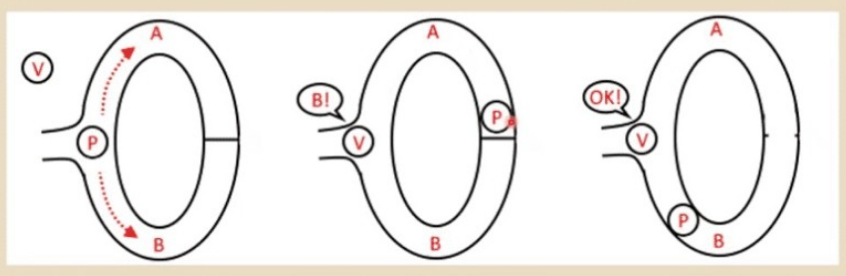
\includegraphics{images/alibaba.png}
   \caption{Here V acknowledges that P knows the secret because he sees P coming out of B}
   \label{fig:alibaba}
\end{figure}

The ``Alibaba's cave'' is a common example to explain ZKPs. In this scenario, a cave has a door that can only be opened by a secret password. A prover wants to convince a verifier that they know the password without revealing it. The prover can open the door and show the verifier that they know the password, but the verifier cannot see the password itself.\\
But what if the prover simply had luck and the door has opened by itself? To avoid this, the prover can repeat the process multiple times, proving to the verifier that they know the password with a high probability.

\subsection{Properties of ZKPs}
\begin{itemize}
   \item \textbf{Completeness}: if the statement is true, the verifier will be convinced by the prover.
   \item \textbf{Soundness}: if the statement is false, the prover will not be able to convince ---easily--- the verifier. 
   \note{its luck will eventually run out}
   \item \textbf{Zero-Knowledge}: the verifier learns nothing about the statement itself.
\end{itemize}

\subsection{Real World and Blockchains}

An interactive protocol is not so useful in the real world, as it often limits the number of potential use-cases of the primitive:
RTTs are expensive and slow, and the prover and verifier would have to be online at the same time.

For what concerns privacy-protected transfers in Blockchains, using ZKPs, it is possible to prove that someone is allowed to spend a certain amount without revealing the sender and receiver address and amount to the whole network.

\section{ZK-SNARKs}

Zero-Knowledge Succinct Non-Interactive Argument of Knowledge (ZK-SNARKs) are a type of ZKP that allows a prover to convince a verifier that a statement is true without revealing any information about the statement itself. ZK-SNARKs are \textbf{non-interactive}, meaning that the prover can generate a proof and send it to the verifier without any interaction.
\begin{itemize}
   \item \texttt{ZK} \textit{Zero-Knowledge}: the verifier learns nothing about the statement itself
   \item \texttt{S} \textit{Succinct}: the proof is short and easy to verify
   \item \texttt{N} \textit{Non-Interactive}: the prover can generate a proof and send it to the verifier without any interaction
   \item \texttt{ARKS} \textit{Argument of Knowledge}: the prover convinces the verifier that the statement is true
\end{itemize}

\section{XACML and ZKPs}
XACML (eXtensible Access Control Markup Language) is a standard for access control that allows administrators to define policies that determine who can access what resources. ZKPs can be used to prove that a user is allowed to access a resource without revealing the user's identity or the resource being accessed.

XACML framework is used in Ethereum to implement access control for smart contracts, 
\begin{itemize}
   \item Outsource the access control decision process
   \item No need of a trusted third party to perform the access control decision
   process
   \item Auditability, decentralization
\end{itemize}

